\documentclass[linenumbers,RNAAS,trackchanges]{aastex631}
\usepackage[utf8]{inputenc}
\usepackage{hyperref}           % hrefs
\usepackage{natbib}             % for bibliography
\usepackage{float}              % figure positioning
\usepackage{svg}                % used for SVG images
\usepackage{tikz}
\usepackage{graphicx}           % used for non-SVG images
\usepackage{amsmath}  

% Search Query Metadata
\shorttitle{Finding minima of Weierstrass functions using the golden section search method}

% Hyperlink setup
\hypersetup{
colorlinks=true,
linkcolor=blue,
urlcolor=blue
}

\tikzset{
  mynode/.style={fill,circle,inner sep=2pt,outer sep=0pt}
}

\begin{document}
\title{Finding minima of Weierstrass functions using the golden section search method}
% [] is for ORCiD
\correspondingauthor{Ryan Charette, Abigail Iovino, Nicholas Davila}
\email{author1@email.com, abigail.iovino@gmail.com, ndavila@utexas.edu}
\author[0000-0000-0000-0000]{Ryan Charette}
\author[0000-0000-0000-0000]{Abigail Iovino}
\author[0000-0000-0000-0000]{Nicholas Davila}
\affiliation{University of Texas at Austin}

% 250 word limit for abstract
\begin{abstract}
In order to the effectiveness of the golden section search for finding minima in functions, we identified two Weierstrass functions and tested the golden sections search on those functions. The golden section search works by "bracketing" an interval and iteratively reducing its size so that the "brackets" approach an extremum or minimum. Testing the effectiveness of the golden section search on a Weierstrass is interesting because they are one of the most extreme examples of non-differentiable functions which make them very suited for testing the limits of the golden section search method. Our experiment resulted in one 'standard' Weierstrass function's minima being found to a tolerance of $10^{-6}$. Our other function did not find a minima, this is due to the function's respective infinite sum, which is discussed more in detail in the paper.
\end{abstract}

% Use astrothesaurus numbers in place of num
% \keywords{keyword 1 (num) --- keyword 2 (num) --- keyword 3 (num)}
\keywords{Weierstrass function (1) --- continuous but nowhere differentiable function (2) --- golden ratio (3) --- golden section search (4) --- fractal curve (5) --- pathalogical functions (6) --- Karl Weierstrass (7) --- root finding (8) --- Euclid's Elements (9) --- Kiefer optimization (10)}
\section{\textbf{Introduction}} \label{sec:intro}
%in your introduction you will research the historical background of this topic and write a summary of the importance of this computation. We want references to papers in published journals not blogs on the internet.

In mathematics, a golden section is said to divide a line into two unequal parts such that the ratio of the whole to the greater equals the ratio of the greater to the lesser. In particular, 
$$\frac{A+B}{A} = \frac{A}{B},$$ 
where $A$ and $B$ are the respective lengths of greater and lesser lengths segments. The name ``golden section’’ is thought to be coined by Martin Ohm in 1835, but the definition regarding proportional segments of a line appears in Book VI of Euclid’s \textit{Elements} \cite{fowler_1982}.\footnote{The most read book in the world after the bible.} 

In 1953, J. Kiefer harnessed the power of the golden section to solve optimization problems in numerical analysis. The existing methods for ``finding’’ extrema relied on the functions being well-behaved (e.g. continuous, differential etc.). By ``find,’’ we mean that the method reduces an interval to a tolerably small size and approximates the desired value: in the words of Kiefer, “the payoff of the computer to nature is the length of this final interval'' \cite{kiefer_1953}. Kiefer's motivation was to find a method that did not rely on such conditions.

The golden section search method works by ``bracketing'' an interval and iteratively reducing its size so that the endpoints or ``brackets" approach an extremum.\footnote{The bisection method is another example of an iterative bracketing method.} Our implementation of the method serves to find a local minimum. The search method uses four values of $x$ to manipulate the interval. Two endpoints, $a$ and $b$ are given as input, and a third point, $c$ is chosen so that it slices the interval between said endpoints to create a golden section:
    \begin{center}
        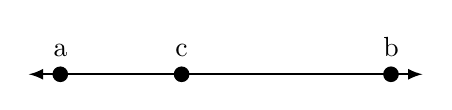
\begin{tikzpicture}
        \draw[black,thick,latex-latex] (0,0) -- (5,0)
        node[pos=.08,mynode,fill=black,label=above:\textcolor{black}{a}]{}
        node[pos=1-.6118,mynode,fill=black,text=blue,label=above:\textcolor{black}{c}]{}
        node[pos=.92,mynode,fill=black,text=green,label=above:\textcolor{black}{b}]{};
      \end{tikzpicture}
    \end{center}
In particular, we take $c$ such $$\frac{|b-a|}{|b-c|} = \frac{|b-c|}{|c-a|}.$$ 
This equation simplifies to $\big|\frac{b-c}{c-a}\big|^2 - \big|\frac{b-c}{c-a}\big| -1 = 0$. We can use the quadratic formula to get that  $\big|\frac{b-c}{c-a} \big|= \frac{1+\sqrt{5}}{2}$. We will denote this value, called the golden ratio, by $\phi$. Using that fact that $\big|\frac{b-c}{c-a} \big|= \phi$ and that $\big|\frac{b-c}{c-a} \big|= \big|\frac{b-a}{b-c} \big|$, we can solve for c: 
    \begin{align*}
        b-a = (b-c)\phi \\
        \frac{b - a -b\phi}{\phi} = -c \\
        \frac{a - b}{\phi} + b = c.
    \end{align*}
Since $c$ creates a golden section where the leftmost segment, the one containing $a$, is the shorter of the two, we can make another golden section where the rightmost segment, the one containing $b$, is the shorter of the two. We call the dividing point $d$, and swap $a$ and $b$ in the equation above to get $d$:
    \[\frac{b - a}{\phi} + a = d\]
Visually,
\begin{center}
    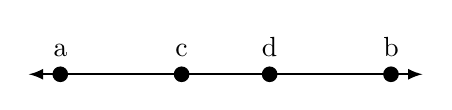
\begin{tikzpicture}
    \draw[black,thick,latex-latex] (0,0) -- (5,0)
    node[pos=.08,mynode,fill=black,label=above:\textcolor{black}{a}]{}
    node[pos=1-.6118,mynode,fill=black,text=blue,label=above:\textcolor{black}{c}]{}
    node[pos=.6118,mynode,fill=black,text=blue,label=above:\textcolor{black}{d}]{}
    node[pos=.92,mynode,fill=black,text=green,label=above:\textcolor{black}{b}]{};
  \end{tikzpicture}
\end{center}
% need help proving this claim:
We claim that $c$ makes a golden section between $a$ and $d$. To verify, we can take $c^*$ such that it forms a golden section between $a$ and $d$ with the rightmost segment being the shorter, and show that $c^* = c$. We have that $c^* = \frac{d-a}{\phi} + a$ and $\frac{d-a}{b-d} = \phi$ (the latter follows from $d$ being a golden ratio between $a$ and $b$). In particular, $\frac{d-a}{\phi} = b-d$. The rest follows from substitution: $$c^* = \frac{d-a}{\phi} + a= b-d+a = b-d + d-\frac{b-a}{\phi} = b + \frac{a-b}{\phi} = c.$$ 
This claim will be crucial to the proof as it reduces the number of calculations and preserves the proportionality of the four points at each iteration. One more verification needs to be made before we can start. The following must hold in order to find a minimum local to (a,b):
\[\bigl(f(c)<f(a) \land f(c)<f(b)\bigr) \lor \bigl(f(d)<f(a) \land f(d)<f(b)\bigr).\]
 To narrow the interval, we first compare $f(c)$ and $f(d)$. If $f(c) < f(d)$,  we make $d$ our new endpoint by shifting $b$ the current $d$ and $d$ to the current $c$:
    \begin{center}
        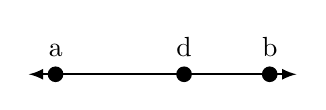
\begin{tikzpicture}
        \draw[black,thick,latex-latex] (0,0) -- (3.4,0)
        node[pos=.10,mynode,fill=black,label=above:\textcolor{black}{a}]{}
        node[pos=.58,mynode,fill=black,text=blue,label=above:\textcolor{black}{d}]{}
        node[pos=.9,mynode,fill=black,text=blue,label=above:\textcolor{black}{b}]{};
      \end{tikzpicture}
      \hspace*{1.3cm}
    \end{center}
Note that $d$ is still a golden section between $a$ and $b$ (refer to the earlier claim). So we need only recalculate $c$ using the new $b$ and repeat the process.

Alternatively, if $f(c) > f(d)$,  we make $c$ our new endpoint shifting $a$ the current $c$ and $c$ to the current $d$:
        \begin{center}
        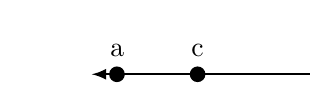
\begin{tikzpicture}
        \hspace*{.8cm}
        \draw[black,thick,latex-latex] (0,0) -- (3.2,0)
        node[pos=.10,mynode,fill=black,label=above:\textcolor{black}{a}]{}
        node[pos=1-.58,mynode,fill=black,text=blue,label=above:\textcolor{black}{c}]{}
        node[pos=.9,mynode,fill=black,text=blue,label=above:\textcolor{black}{b}]{};
      \end{tikzpicture}
    \end{center}
    
\noindent
Again, $c$ maintains the golden ratio, so we recalculate $d$ with our new $a$ and repeat the process. At each iteration, we decrease the interval length by $\frac{1}{\phi}$, always maintaining the desired proportions between our four points. We continue until $|f(c) - f(d)|$ is smaller than some tolerance.\\

\noindent
You will notice that the method does not take any derivatives. Therefore, the method is particularly useful for finding extrema of continuous functions that are not everywhere differentiable. A classic example of such a function is a Weierstrass function, which famously serves as a counterexample against notions of continuity implying differentiability, since it continuous everywhere but differentiable nowhere.

\vspace{1cm}
\section{\textbf{function choice statement}}
% Write why the equations matters (to you or other people) and what the equation is.
The problem that we are attempting to solve is the numerical approximation of minima on non-differentiable functions. In order to find extrema without the use of calculus, we first use a graphical approach to find a reasonable interval on which we are confident that there exists a minimum. Via the golden search algorithm, we are able to narrow this interval to a reasonable tolerance. The functions we chose are Weierstrass function, which are continuous everywhere but differentiable nowhere. These functions were selected because they are the most extreme examples of non-differentiable functions, and as such are especially well-suited to this method of determining minima. Additionally, Weierstrass functions are useful in physics for the approximation of processes that are randomly determined, such as Brownian motion.

The functions analyzed are:
\begin{equation}
    f_1(x) = \sum_{n = 0}^{20}\frac{1}{2^n} \cos{(3^n \pi x)}
\end{equation}
\begin{equation}
    f_2(x) = \sum_{n = 0}^{20} \frac{1}{2^n} \sin{(2^nx)}
\end{equation}
A graphical rendering of each is below:
\begin{figure}[H]
 \centering
 \includegraphics[width=0.55\textwidth]{W_alpha1_plot.png}
 \caption
 {\protect Plot for the $\displaystyle \lim_{n \to \infty} \frac{1}{2n} \cos{(3^n \pi x)}$ Weierstrass function. 
 %We are calling this one our function 1.
 }
 \label{fig:apparatus}
\end{figure}
\begin{figure}[H]
 \centering
 \includegraphics[width=0.55\textwidth]{W_alpha2_plot.png}
 \caption
 {\protect Plot for the $\displaystyle \lim_{n \to \infty} \frac{1}{2n} \sin{(2^n x)}$ Weierstrass function. 
 %We are calling this one our function 2.
 }
 \label{fig:apparatus}
\end{figure}

\section{\textbf{results}}
%You will present your results in the form of a table.
\begin{table}[H]
    \centering
    \begin{tabular}{|c|c|c|}
         \hline
         Iterations &  a & b \\
         \hline
         0 & 0 & 2 \\
         \hline
         1 & 0.7639320 & 1.236068 \\
         \hline
         2 & 0.9442719 & 1.055728 \\
         \hline
         3 & 0.9868444 & 1.013156 \\
         \hline
         4 & 0.9968944 & 1.003106 \\
         \hline
         5 & 0.9992669 & 1.000733 \\
         \hline
         6 & 0.9998269 & 1.000173 \\
         \hline
         7 & 0.9999591 & 1.000041 \\
         \hline
         8 & 0.9999904 & 1.000010 \\
         \hline
         9 & 0.9999977 & 1.000002 \\
         \hline
         10 & 0.9999995 & 1.000001 \\
         \hline
         11 & 0.9999999 & 1.000000 \\
         \hline
    \end{tabular}
    \caption{Our results for running a golden section search on the Weierstrass function which can be seen in Figure 1. Our results have been reduced to 7 significant figures for the sake of readability. We used a tolerance of $10^{-6}$.}
    \label{tab:data_tab}
\end{table}

\begin{table}[H]
    \centering
    \begin{tabular}{|c|c|c|}
         \hline
         Iterations &  a & b \\
         \hline
         0 & -2 & 0 \\
         \hline
         1 & -1.236068 & -0.7639320 \\
         \hline
         2 & -1.055728 & -0.7639320 \\
         \hline
         3 & -0.9442719 & -0.8753882 \\
         \hline
         4 & -0.9179607 & -0.8753882 \\
         \hline
         5 & -0.9016994 & -0.8916494 \\
         \hline
    \end{tabular}
    \caption{Our results for running a golden section search on the Weierstrass function which can be seen in Figure 2. Our results have been reduced to 7 significant figures for the sake of readability. We used a tolerance of $10^{-6}$.} As mentioned in the error section, sometimes the algorithm terminates early, and 
    \label{tab:data_tab}
\end{table}
%\subsection{Error plot}






\section{\textbf{results interpretation and error discussion}}
Both functions (1) and (2) are approximations of their respective infinite sums. Because the $\lim_{n \to \infty} \frac{1}{2n} \cos{(3^n \pi x)}$ and the  $\lim_{n \to \infty} \frac{1}{2n} \sin{(2^n x)}$ both do not exist, their sums are divergent. Thus, the remainder between the infinite sums and their first 20 terms can not be exactly determined. Further, the finite sums are not infinitely self-similar, so as the algorithm focuses on a tighter interval, the functions lose detail. As such, despite Weierstrass functions containing a minimum on all intervals, the algorithm sometimes terminates without finding a minimum on small intervals. In this case, the algorithm returns the smallest interval on which it was able to determine that a minimum exists.

\section{\textbf{Conclusion}} \label{sec:summary}
Via the golden search algorithm, we were able to identify minima on Weierstrass functions. Additionally, the algorithm developed is shown mathematically to work on other functions as well. Due to the truncation of infinite series however, errors occur as the tolerance decreases.

\section{\textbf{Acknowledgment}} \label{sec:acknowledgment}
Ryan, Abi, and Nick would like to thank Brett for his timely manner and thoroughness when answering all of our questions, even in non-working hours. We would also like to thank Professor Mitra for his guidance and support. 

\newpage
\bibliographystyle{aasjournal}
\bibliography{bibliography.bib}

\end{document}
